\documentclass[border=10pt]{standalone}
\usepackage{graphicx}
\usepackage{tikz}
\usepackage{xcolor}
\usetikzlibrary{arrows.meta, positioning, fit, backgrounds, shapes.geometric}
\definecolor{academicblue}{RGB}{30,64,105}
\definecolor{accent}{RGB}{180,120,40}
\definecolor{muted}{RGB}{100,116,139}
\begin{document}
\resizebox{16.5cm}{!}{%
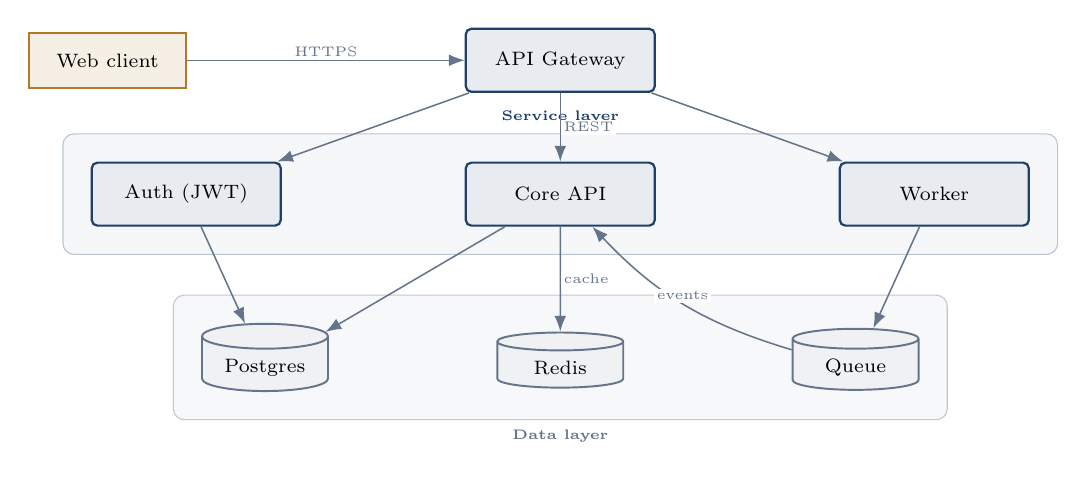
\begin{tikzpicture}[
  font=\scriptsize,
  svc/.style={rectangle, rounded corners=2pt, draw=academicblue, line width=0.8pt,
    fill=academicblue!10, minimum width=2.4cm, minimum height=0.8cm, align=center},
  store/.style={cylinder, shape border rotate=90, draw=muted, line width=0.7pt,
    fill=muted!10, minimum width=1.6cm, minimum height=0.7cm, align=center, aspect=0.25},
  client/.style={rectangle, draw=accent, line width=0.8pt, fill=accent!12,
    minimum width=2cm, minimum height=0.7cm, align=center},
  arr/.style={-{Latex[length=2mm]}, draw=muted, line width=0.55pt},
  lbl/.style={font=\tiny, text=muted, midway, fill=white, inner sep=1pt}
]
\node[client] (web) at (2.5,2.6) {Web client};
\node[svc] (gw) at (8.25,2.6) {API Gateway};
\node[svc] (auth) at (3.5,0.9) {Auth (JWT)};
\node[svc] (core) at (8.25,0.9) {Core API};
\node[svc] (worker) at (13,0.9) {Worker};
\node[store] (db) at (4.5,-1.3) {Postgres};
\node[store] (cache) at (8.25,-1.3) {Redis};
\node[store] (queue) at (12,-1.3) {Queue};
\begin{scope}[on background layer]
  \node[draw=academicblue!30, rounded corners=4pt, fill=academicblue!4,
    inner sep=10pt, fit=(auth)(core)(worker), label={[font=\tiny\bfseries, text=academicblue]above:Service layer}] {};
  \node[draw=muted!40, rounded corners=4pt, fill=muted!5,
    inner sep=10pt, fit=(db)(cache)(queue), label={[font=\tiny\bfseries, text=muted]below:Data layer}] {};
\end{scope}
\draw[arr] (web) -- node[lbl, above] {HTTPS} (gw);
\draw[arr] (gw) -- (auth);
\draw[arr] (gw) -- node[lbl, right] {REST} (core);
\draw[arr] (gw) -- (worker);
\draw[arr] (auth) -- (db);
\draw[arr] (core) -- (db);
\draw[arr] (core) -- node[lbl, right] {cache} (cache);
\draw[arr] (worker) -- (queue);
\draw[arr] (queue) to[bend left=15] node[lbl, above] {events} (core);
\end{tikzpicture}%
}
\end{document}
